\begin{figure}[t]
    \centering
    \begin{subfigure}[t]{0.31\textwidth}
    \centering
        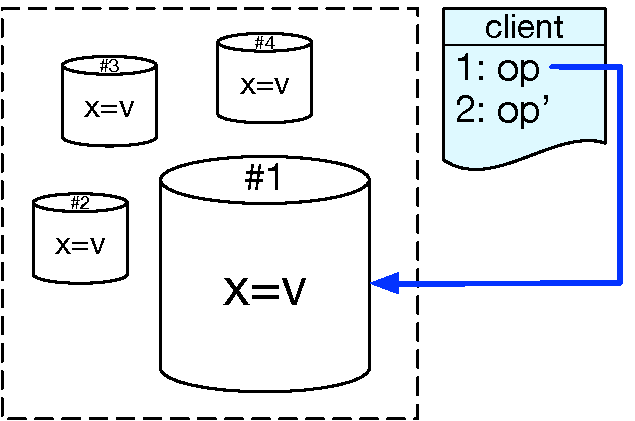
\includegraphics[scale=0.36]{Figures/system_model1.pdf}
        \caption{A client submits an operation op to the store, which
	is routed to the replica1.}
        \label{fig:sys_model1}
    \end{subfigure}
    \hfill
    \begin{subfigure}[t]{0.31\textwidth}
        \centering
	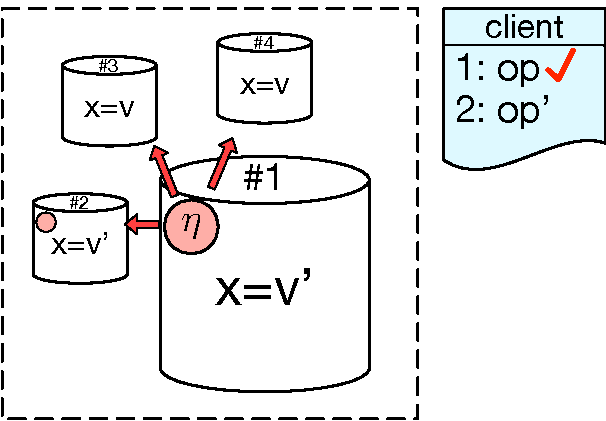
\includegraphics[scale=0.36]{Figures/system_model2.pdf}
        \caption{The state of the object at replica1 is updated, an
	effect is created and is being propagated.}
        \label{fig:sys_model2}
    \end{subfigure}
    \hfill
    \begin{subfigure}[t]{0.31\textwidth}
        \centering
	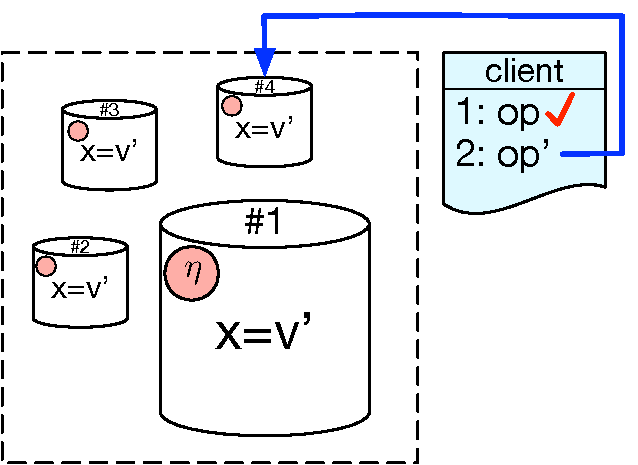
\includegraphics[scale=0.36]{Figures/system_model3.pdf}
        \caption{second operation op' is submitted to the store, which
	is this time routed to the replica4.}
        \label{fig:sys_model3}
    \end{subfigure}
    \caption{system model of \tool}\label{fig:system_model}
\end{figure}
